\section{Numerical Results}

\begin{frame}{Numerical Results, c.f.~\href{https://github.com/TiKeil}{github.com/TiKeil}}
    \only<1>{
        \begin{figure}
            \begin{center}
                \includegraphics[height=0.42\textheight]{room_diffusivity.png}
                \includegraphics[height=0.42\textheight]{room_heaters.png}
                \includegraphics[height=0.42\textheight]{room_to_heat.png}
            \end{center}
        \end{figure}
    }

    \only<2>{
        \begin{figure}
            \includegraphics[height=0.7\textheight]{solution.png}
        \end{figure}
    }
\end{frame}

\begin{frame}{Numerical Results, c.f.~\cite{Keil2021}, data courtesy of Tim Keil}
    \begin{figure}
        \centering
        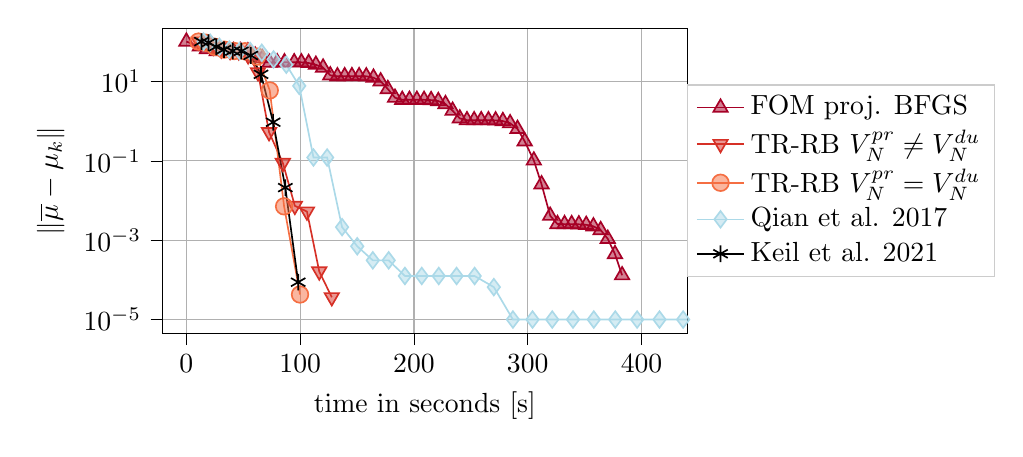
\begin{tikzpicture}[>=stealth]
            \definecolor{color0}{rgb}{0.65,0,0.15}
            \definecolor{color1}{rgb}{0.84,0.19,0.15}
            \definecolor{color2}{rgb}{0.96,0.43,0.26}
            \definecolor{color3}{rgb}{0.99,0.68,0.38}
            \definecolor{color4}{rgb}{1,0.88,0.56}
            \definecolor{color5}{rgb}{0.67,0.85,0.91}
            
            \begin{axis}[
            width=0.68\linewidth,
            height=0.45\linewidth,
            name=right,
            legend cell align={left},
            legend style={fill opacity=0.8, draw opacity=1, text opacity=1, at={(1,0.5)}, anchor=west, draw=white!80!black},
            log basis y={10},
            tick align=outside,
            tick pos=left,
            x grid style={white!69.0196078431373!black},
            xlabel={time in seconds [s]},
            xmajorgrids,
            xmin=-20.960649907589, xmax=440.173648059368,
            xtick style={color=black},
            y grid style={white!69.0196078431373!black},
            ylabel={\(\displaystyle \| \overline{\mu}-\mu_k \|\)},
            ymajorgrids,
            ymin=4.4843436808366e-06, ymax=220.993014467563,
            ymode=log,
            ytick style={color=black}
            ]
            \addplot [semithick, color0, mark=triangle*, mark size=3, mark options={solid, fill opacity=0.5}]
            table [row sep=crcr]{%
                0 101.694749908925\\
                11.8227753639221 76.6344328826546\\
                18.0333218574524 65.5067669990911\\
                26.6583814620972 58.1295253774286\\
                35.0693249702454 59.0115951280537\\
                41.360090970993 58.4939381433727\\
                47.6699612140656 58.3395819689597\\
                54.0571613311768 57.4951884391855\\
                60.475839138031 44.9083655387143\\
                66.8279640674591 38.7433342505646\\
                73.1730172634125 30.1132884189381\\
                79.8124206066132 30.541943990057\\
                86.1816501617432 30.5797403707051\\
                94.744637966156 30.6877367833582\\
                101.086725711823 30.5139572509563\\
                107.417257547379 29.3771285500316\\
                113.785773038864 26.5388565600953\\
                120.147310733795 22.560037310177\\
                126.465299129486 14.3479859523988\\
                132.743663549423 13.5804698329301\\
                139.105927705765 13.6677252430272\\
                145.466085195541 13.6854911537257\\
                151.809690237045 13.6702499690576\\
                158.101904153824 13.5504640651469\\
                164.427534341812 12.5237935862747\\
                170.725522756577 10.1390172370278\\
                177.048982620239 6.47893809307185\\
                183.360107898712 3.91162947760179\\
                189.69978260994 3.46480482852387\\
                196.036733865738 3.46586360401667\\
                202.56974029541 3.46694944167388\\
                208.870253324509 3.46012010437098\\
                215.07564496994 3.40591532107205\\
                221.397597789764 3.22469574742039\\
                227.699336051941 2.70155535774846\\
                233.960841655731 1.84053812825313\\
                240.292472839355 1.17557279387446\\
                246.58556842804 1.05901236143825\\
                252.882767438889 1.06020275336439\\
                259.096759080887 1.0611800350202\\
                265.451264858246 1.0603964339395\\
                271.741575241089 1.05006611015456\\
                278.136191129684 1.00745053958016\\
                284.483489274979 0.890082498254083\\
                290.997215986252 0.639372370454038\\
                297.312686681747 0.311869643001277\\
                305.364391565323 0.102122548506474\\
                312.132185220718 0.0256872520461831\\
                319.721675395966 0.00413078425544472\\
                326.131166934967 0.00255412308842596\\
                332.34970498085 0.00254610141212139\\
                338.603756427765 0.0025429009369023\\
                344.915750026703 0.0025127226206382\\
                351.409331083298 0.0024398138461593\\
                357.721709489822 0.00223763288468792\\
                364.101721763611 0.00179700448435439\\
                370.322831630707 0.00108508397827876\\
                376.664766073227 0.000445536313619211\\
                382.943562269211 0.000130715792809606\\
            };
            \addlegendentry{FOM proj. BFGS}
            \addplot [semithick, color1, mark=triangle*, mark size=3, mark options={solid,rotate=180, fill opacity=0.5}]
            table [row sep=crcr]{%
                10.9836044311523 101.694749914018\\
                17.0856072902679 95.2544133844278\\
                23.7086544036865 75.4099308159367\\
                30.5910837650299 64.0679273362064\\
                38.4077038764954 58.8254086036674\\
                46.041802406311 57.9178213150213\\
                54.2439885139465 45.7674046218088\\
                62.901976108551 17.1659141983604\\
                72.6504902839661 0.528120998554676\\
                84.7693104743958 0.088572996002305\\
                95.3249473571777 0.00733824299393689\\
                105.960053682327 0.00527301821282116\\
                116.768208503723 0.000162636786332236\\
                127.789884090424 3.64077041750881e-05\\
            };
            \addlegendentry{TR-RB $V_N^{pr} \neq V_N^{du}$}
            \addplot [semithick, color2, mark=*, mark size=3, mark options={solid, fill opacity=0.5}]
            table [row sep=crcr]{%
                10.6433067321777 101.694749914018\\
                17.1916410923004 95.0951073301147\\
                24.9593110084534 75.0102498060299\\
                33.0756437778473 63.7333999506352\\
                42.0009367465973 58.8433158089068\\
                51.5410561561584 58.0198982797859\\
                62.0700180530548 42.5520357574727\\
                73.2681591510773 5.97831025727406\\
                85.8639888763428 0.00714132377950299\\
                99.8546583652496 4.2715167840283e-05\\
            };
            \addlegendentry{TR-RB $V_N^{pr} = V_N^{du}$}
            \addplot [semithick, color5, mark=diamond*, mark size=3, mark options={solid, fill opacity=0.5}]
            table [row sep=crcr]{%
                15.0834636688232 101.694749914018\\
                20.8926212787628 95.2544133844278\\
                29.018415927887 75.4099308159367\\
                37.7143726348877 64.0679273362064\\
                46.7216105461121 58.9002429218621\\
                56.0600709915161 58.7665520191065\\
                66.2690076828003 53.1967067086869\\
                76.5717370510101 36.1345643809206\\
                87.8098843097687 26.5812213583053\\
                99.1848306655884 7.77184075151648\\
                111.681534767151 0.121698707208084\\
                123.707145929337 0.12139085075229\\
                136.807378292084 0.00213458006709451\\
                150.148610115051 0.00070265838616608\\
                163.837367534637 0.000310413647634123\\
                177.788628339767 0.000310251084753871\\
                192.031569719315 0.000125322245049535\\
                206.855760335922 0.000125272954182688\\
                221.766639947891 0.000125185538394569\\
                237.465733289719 0.000125184171346979\\
                253.313305139542 0.00012501858548298\\
                270.196664571762 6.56715239340949e-05\\
                286.975438117981 9.98241579955393e-06\\
                304.209729194641 9.98109460785684e-06\\
                321.546380996704 9.98107397048428e-06\\
                339.791335582733 9.98107396716918e-06\\
                358.050210237503 9.98090889164456e-06\\
                376.922388076782 9.98090760207332e-06\\
                396.134050607681 9.98090756246715e-06\\
                415.789769649506 9.98082502525526e-06\\
                436.588827371597 9.98082486641714e-06\\
                455.848903417587 9.98082486641714e-06\\
                475.412249565125 9.98082486641714e-06\\
                496.140789747238 9.98082486641714e-06\\
                514.43416762352 9.98082486641714e-06\\
                532.975608110428 9.98082486641714e-06\\
                551.482770204544 9.98082486641714e-06\\
                571.509459733963 9.98082486641714e-06\\
                590.078435897827 9.98082486641714e-06\\
                608.564557790756 9.98082486641714e-06\\
                627.022351980209 9.98082486641714e-06\\
            };
            \addlegendentry{Qian et al. 2017}
            \addplot [semithick, black, mark=asterisk, mark size=3, mark options={solid, fill opacity=0.5}]
            table [row sep=crcr]{%
                13.2413511276245 101.694749914018\\
                19.3898150920868 95.2544133844209\\
                26.1817166805267 75.3587869929344\\
                33.0169637203217 63.9788199949804\\
                40.6761891841888 58.859685583101\\
                48.2365906238556 58.2492967427756\\
                56.5340046882629 45.4725937425856\\
                65.5767681598663 15.1974212649069\\
                76.236855506897 0.942934319070116\\
                86.953501701355 0.021167321405947\\
                98.2464504241943 8.72644160303025e-05\\
            };
            \addlegendentry{Keil et al. 2021}
            \end{axis}
        \end{tikzpicture}
    \end{figure}
\end{frame}